\documentclass[12pt]{article} % use larger type; default would be 10pt
\usepackage[utf8]{inputenc} % set input encoding (not needed with XeLaTeX)

%%% PAGE DIMENSIONS
\usepackage{geometry} % to change the page dimensions
\geometry{a4paper} % or letterpaper (US) or a5paper or....
\geometry{margin=2cm} % or letterpaper (US) or a5paper or....

\usepackage{graphicx} % support the \includegraphics command and options
\usepackage[parfill]{parskip} % Activate to begin paragraphs with an empty line rather than an indent
\usepackage{times} % for Times Roman default font

%%% PACKAGES
\usepackage{booktabs} % for much better looking tables
\usepackage{array} % for better arrays (eg matrices) in maths
\usepackage{paralist} % very flexible & customisable lists (eg. enumerate/itemize, etc.)
\usepackage{verbatim} % adds environment for commenting out blocks of text & for better verbatim
\usepackage{subfig} % make it possible to include more than one captioned figure/table in a single float

%%% HEADERS & FOOTERS
\usepackage{fancyhdr} % This should be set AFTER setting up the page geometry
\pagestyle{fancy} % options: empty , plain , fancy
\renewcommand{\headrulewidth}{0pt} % customise the layout...
\lhead{}\chead{}\rhead{}
\lfoot{}\cfoot{\thepage}\rfoot{}

\makeatletter
\renewcommand{\maketitle}{%
  {\bfseries{\scshape{\Large{\@title\par}}}}
}
\makeatother

\hyphenation{Kiwi-bank} % otherwise it may get hyphenated as Ki-wibank

%%% END Article customizations

%%% The "real" document content comes below...

\title{Lake Man Biv Recce: 2-3 September 2017}

\begin{document}
  \maketitle
We left the car just before the rise going over the Poplars Range spur north of the Engineers Camp, and started walking about 13:30.  Crossing the Boyle was easy, but cold, and we continued along the Tui Track in our 'river shoes' (for Robyn an old pair of boots, for me crocs) until after we had crossed the Doubtful, which we did about 1$\frac{1}{2}$ kilometres upstream from its confluence with the Boyle.

Doubtful Hut, which we reached after about 3 hours, has been recently renovated by the NZDA.  It currently has no fire, but there are plans to install a twig burner this summer.  It is in a lovely setting (plagued with sandflies in the summer apparently), and has three bunks (but only two mattresses).

\begin{figure}[ht]
%\centering
\begin{minipage}{.5\linewidth}
\begin{flushleft}
   \includegraphics[width=8cm]{LakeManBivRecce2Sep2017Photo1}
   \captionof{figure}{Doubtful Hut}
\end{flushleft}
\end{minipage}
\begin{minipage}{.5\linewidth}
\begin{center}
   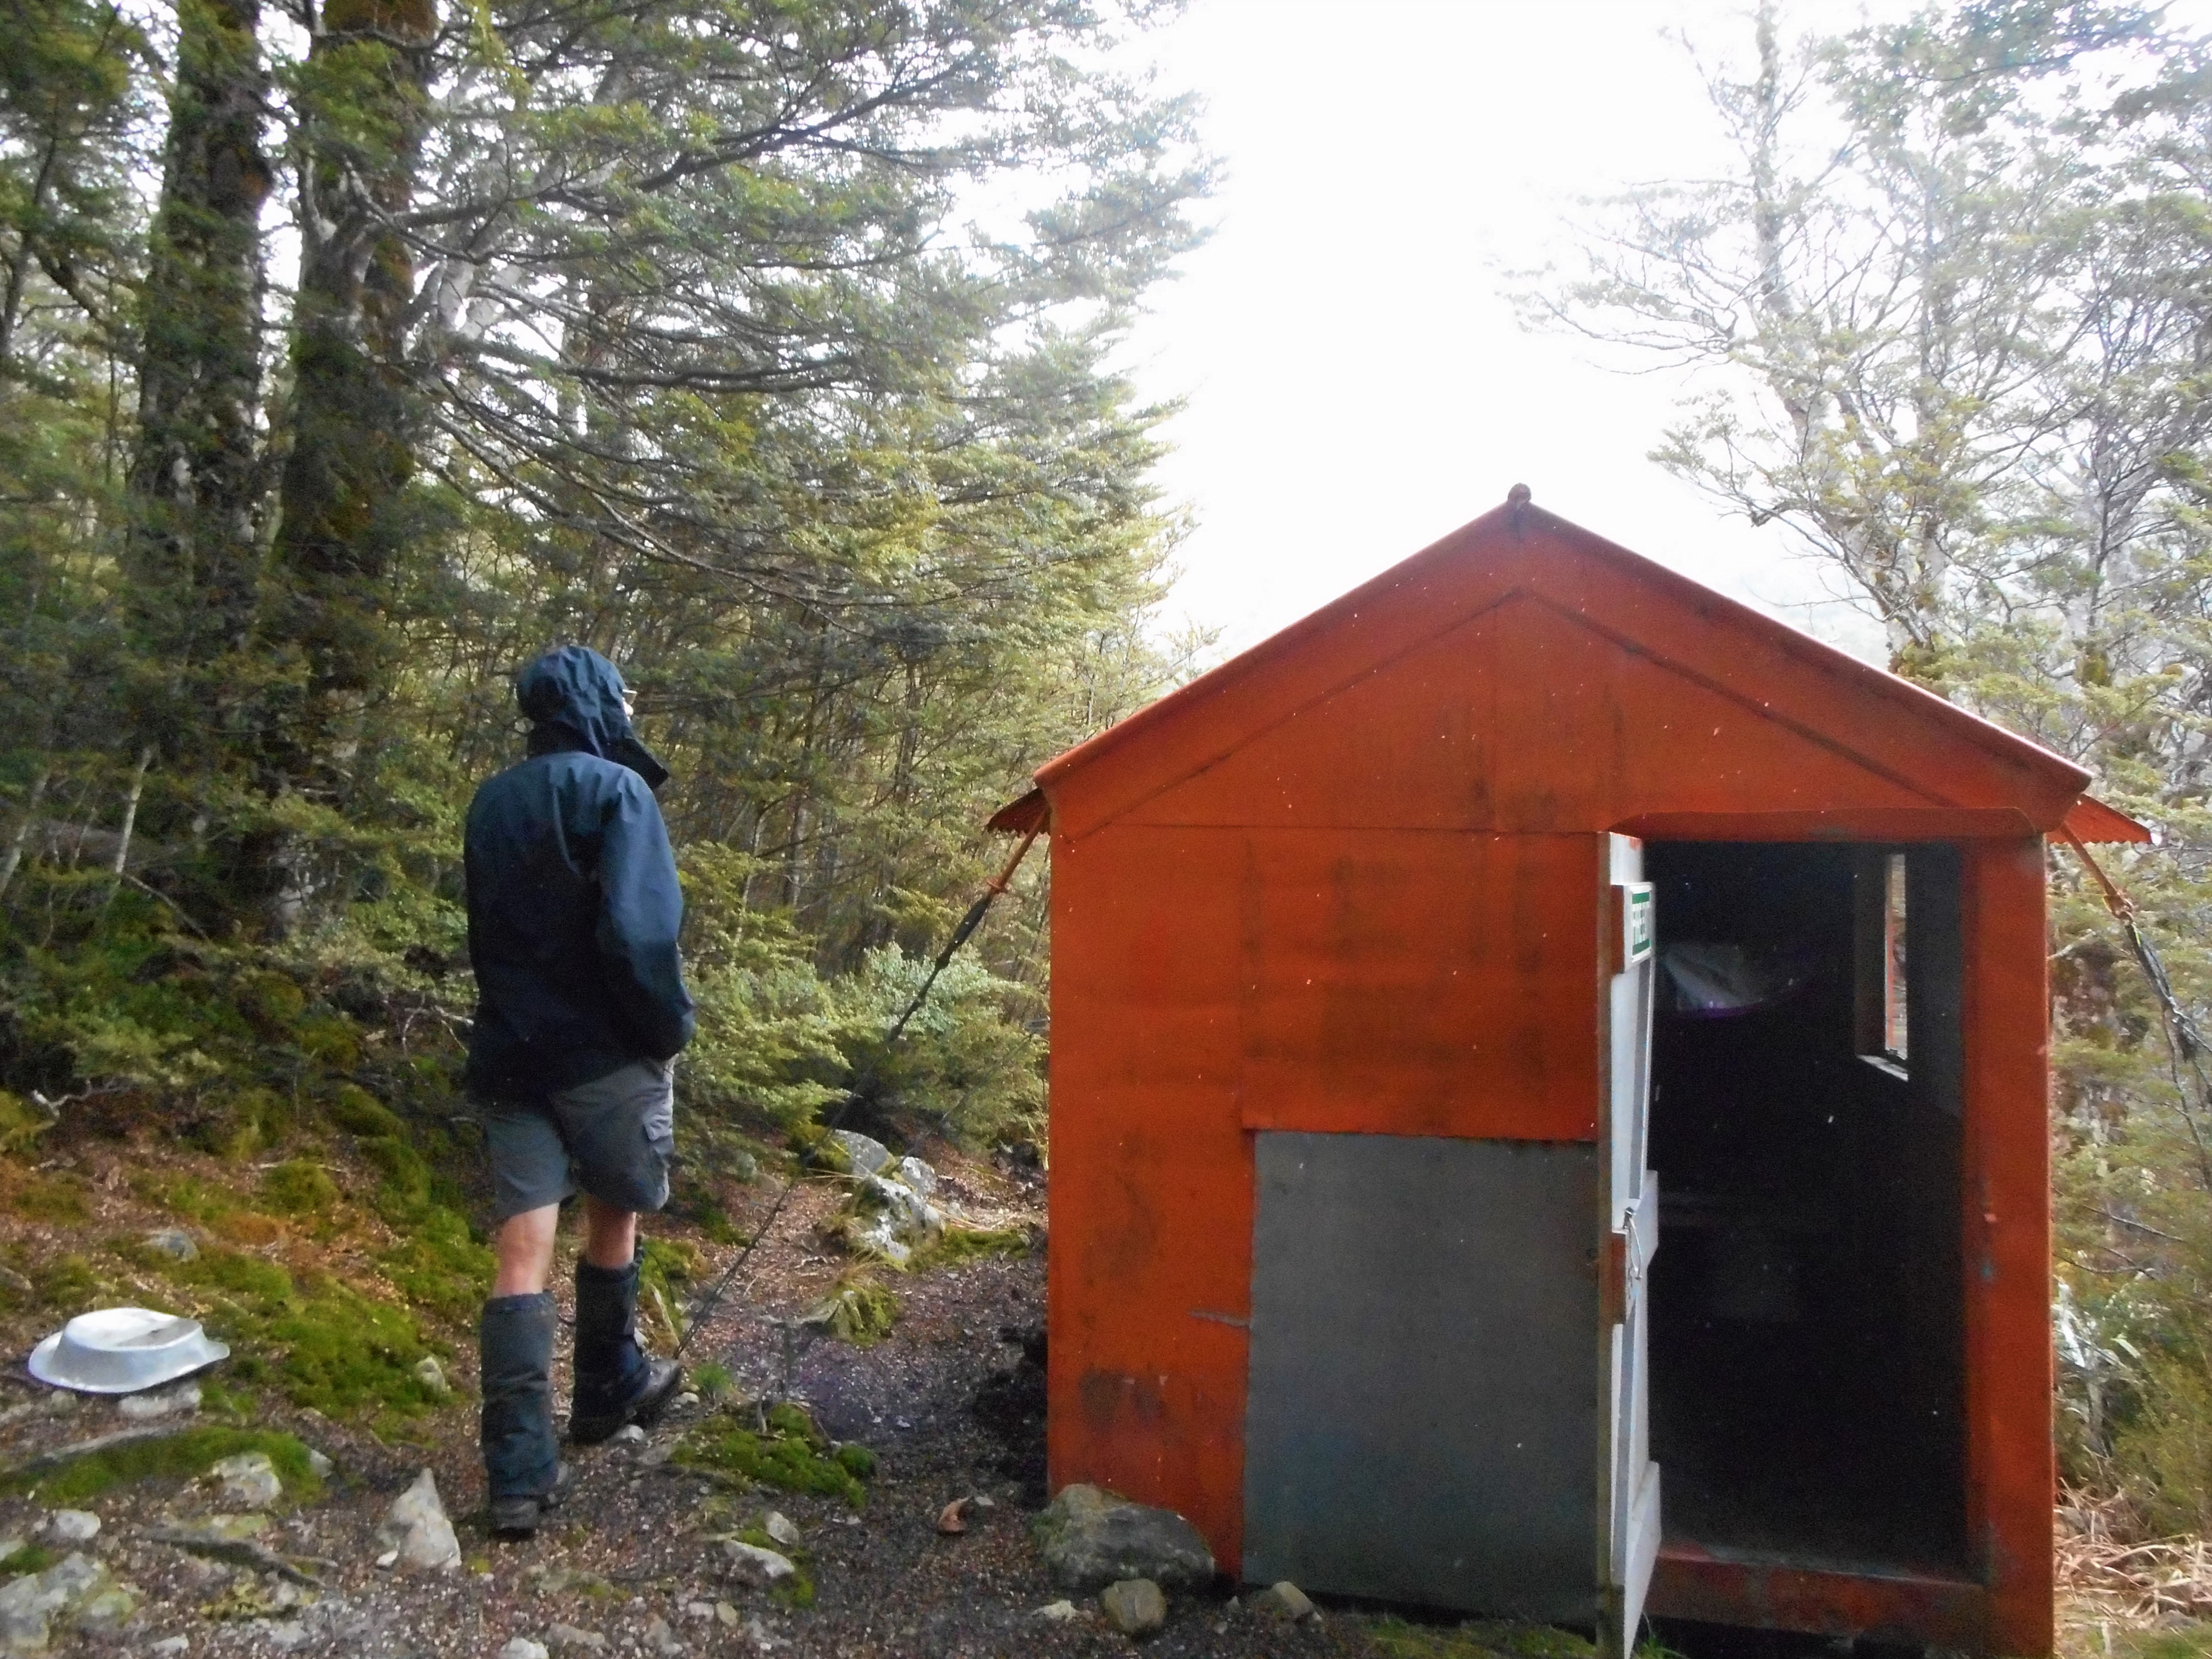
\includegraphics[width=8cm, angle=270]{LakeManBivRecce2Sep2017Photo2}
   \captionof{figure}{Lake Man Biv}
\end{center}
\end{minipage}
\end{figure}

The following day we did a day-walk to Lake Man Biv.  This took a little under 3 hours.  The biv is in pretty good condition (much the same a Lucretia) - much better than I remember.  The bunks, of which there are two, are stretched canvas.  We made notes for a report to DoC, had lunch, and returned to Doubtful Hut.  As we reached this before 15:00, Robyn decided it would be a good idea to continue out.  As we were packing a member of NZDA and his young son arrived - it was from him that we learnt of the intention to install a twig burner.  Walking out was very pleasant and we reached the car just before dusk.

\begin{figure}[ht]
%\centering
\begin{minipage}{.5\linewidth}
\begin{flushleft}
   \includegraphics[width=8cm]{LakeManBivRecce2Sep2017Photo3}
   \captionof{figure}{Mt Lakeman}
\end{flushleft}
\end{minipage}
\begin{minipage}{.5\linewidth}
\begin{flushright}
   \includegraphics[width=8cm]{LakeManBivRecce2Sep2017Photo4}
   \captionof{figure}{Doubtful valley, heading out}
\end{flushright}
\end{minipage}
\end{figure}

\begin{flushright}
Robyn, Peter and dog
\end{flushright}

\end{document}
